This thesis details a control method to perform setpoint regulation for a soft robotic actuator. The proposed method combines classic control theory with additional control methods to fit the purpose of controlling soft robots. This introductory chapter provides context in which this research is performed. First, a detailed description of soft robots is provided. Illustrations of already developed soft robots are included. Furthermore, parallels and differences are drawn between soft robots and classic rigid robots. This helps to understand the need for new control methodologies for solving control problems applied to soft robots. This chapter is concluded by detailing the research outline and its research objectives.


\section{Background}



\subsection{Introduction to soft robotics}

In recent years, the field of soft robotics has received a substantial increase of interest. Soft robots reshape the idea of using robots for industrial processes. Currently, rigid robots dominate the field of industrial automation. As they excel in accuracy, repeatability and load capacity. However, these robots tend to be unsafe to operate in human-centred environments. Classic robots are made from rigid material and accelerate to high velocities, creating a dangerous setting for humans. Additionally, these robots have limited degrees of freedom, making it harder to avoid obstacles. To evade the risks of potential harm, soft robots are made from flexible material. Furthermore, their inherently dexterous structure allows soft robots to move around obstacles. This makes soft robots robust in constantly changing environments. The foundation of soft robotic design is often found in nature. This includes inspiration for material, locomotion, and morphology. A few examples of bio-inspired soft robots include emulated trunks \cite{hannan2003kinematics} inspired by the proboscis of an elephant, robots based on the arm of octopus \cite{wang2013visual}, and robots that replicate the movement of fish \cite{marchese2014}. Figure (\ref{fig1:softexample}) shows a few experimental soft robots. 


\begin{figure}[H]       
    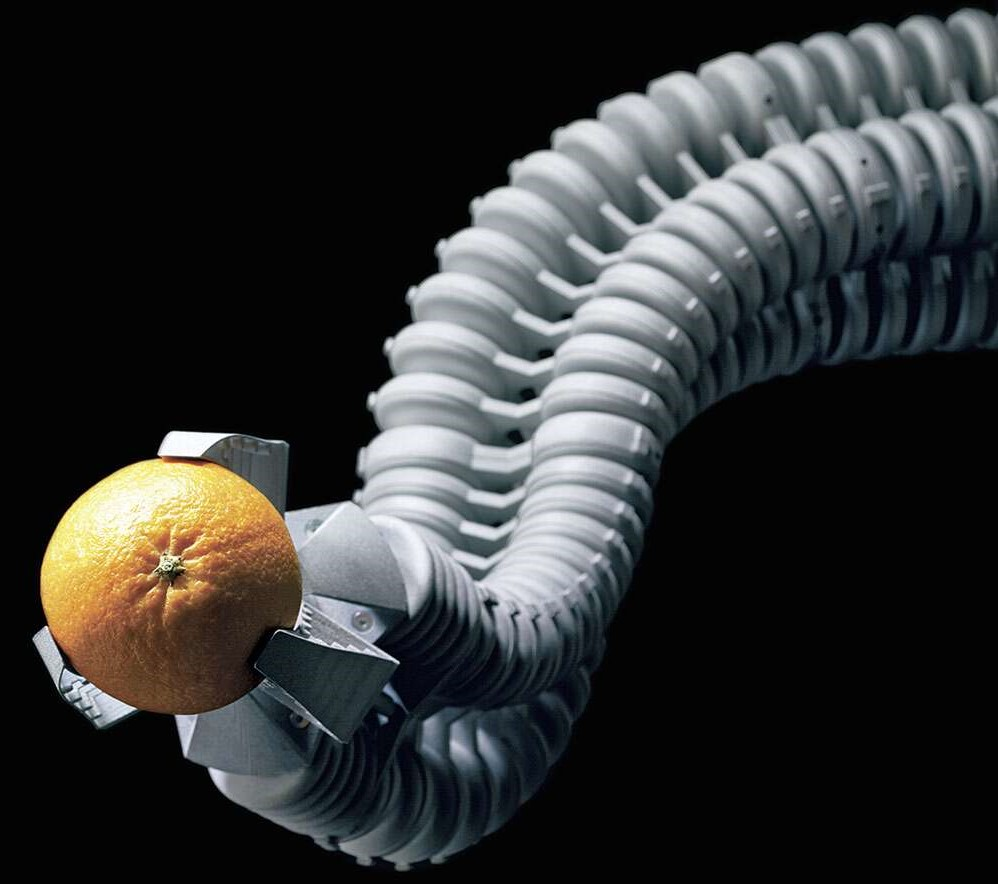
\includegraphics[width = 0.3\textwidth]{Figures/Introduction/bhasinasappel.jpg}   
    \hspace{0px}
    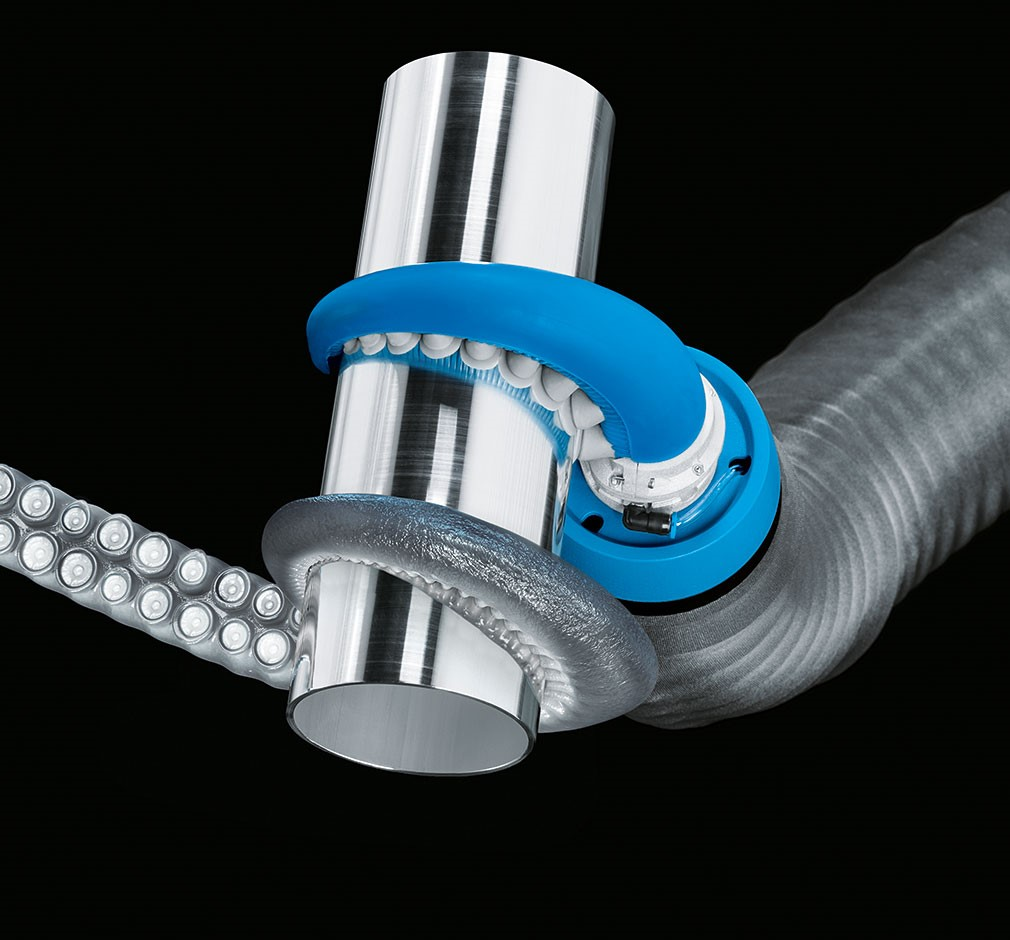
\includegraphics[width = 0.3\textwidth]{Figures/Introduction/tentaclegripper.jpg}
    \hspace{0px}
    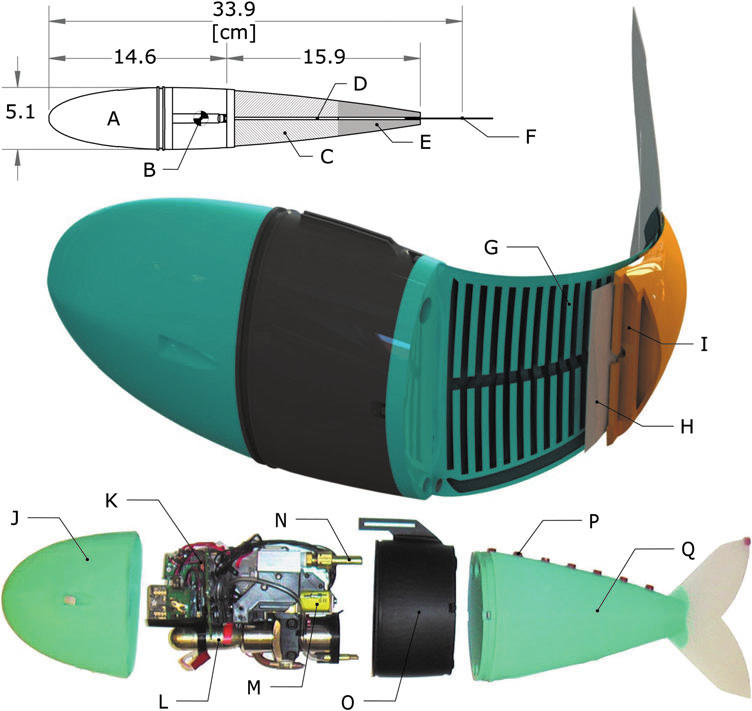
\includegraphics[width = 0.3\textwidth]{Figures/Introduction/fish.jpg}
    \caption{From left to right. Bionic Handling Assistant inspired by the trunk of an elephant \cite{BHA}. Octopus-inspired robot able to move and manipulate a wide range of objects \cite{octopus}.Bio-inspired soft robot replicating movement of a fish \cite{marchese2014}.}
    \label{fig1:softexample}
\end{figure}

There are some major differences between soft robots and the common rigid robots. The first notable difference is the robots' compliance of their underlying materials. Soft robots are inherently compliant and undergo large deformation during regular operation. As a result of this compliance, gravity and payload cause a distributed deformation throughout the entire system \cite{trivedi2008soft}. Theoretically, this gives the robot an infinite amount of degrees of freedom. For a desired end-effector position in three dimensional workspace, the soft robot can take infinitely many configurations. This leads to non-unique solutions. On the contrary, traditional robots are often kinematically non-redundant. This implies that each joint is used to control an additional degree-of-freedom. The soft robots redundancy allows operation in unstructured and changing environments. Robot actuation and sensing is another major difference between the two robot types. Rigid robots are often linked by rotatory or prismatic joints. Each of these joints are mechanically actuated using electric motors. Furthermore, this design also allows to incorporate encoders used to measure rotation. The majority of soft robots is pneumatically actuated \hl{citation}. This actuation method introduces more dynamics into account when actuating the sytem. Other options to actuate the system 

Since soft robots lacks physical joints to place sensors, position sensing is more cumbersome. In previous research vision systems, IMU, \hl{piezo-sensors, meer examples en references} are used. 

Apart from compliance, robot actuation 


under load effects and gravity.  

will result in a distributed deformation under the effects of load and gravity. 

This causes the robot to 

A soft robot is inherently compliant and exhibits
large strains in normal operation

Whereas rigid robots generally consist of multiple rigid sections linked together

links that have mechanical actuators inside the joints. Each of this joint controls an additional DOF. A mechanical system is considered redundant if it has more degrees of freedom than those strictly required to execute a given task \cite{chiaverini2016redundant}. Opposed to rigid robots, bio-inspired robots do not necessarily have these links, and are therefore called continuum robots. Due to there continuous morphology, these robots are inherently redundant. Bio-inspired continuum robots can generally be classified into two categories namely, hard continuum robots and soft continuum robots. In general, hard continuum robots consist of rigidly linked vertebrates that form the backbone of the soft robot. This backbone is compliant resulting in a smooth deformation of the robot when external load is applied. An example is the elephant trunk's robot \cite{cieslak1999elephant}, which consists of eight elastic segments linked together by coil springs. Each segment has two pairs of strings that can control the movement of each individual segment. Servo or linear actuators can be use to wind and unwind the strings with that controlling the movement of the robot, these are so called tendon-driven robots. Soft continuum robots are commonly composed of materials, whose mechanical strength is close to those of biological materials such as, muscles, skin, cartilage, and have a Young's modulus of around 1 gigapascal \cite{rus2015design}. Soft robots are generally pneumatically actuated, an example is the Bionic Handling Assistant (BHA) \cite{rolf2012constant} as shown in Figure \ref{fig:BHA}. By inflating chambers this robot is able to extend and bend. Soft robots are commonly highly dexterous, enabling them grasp objects around obstacles. There are multiple challenges with regards to controlling soft robots. Due to its inherently flexible nature, heavy loads at the end-effector can cause deformation throughout the whole mechanical structure of the robot. Furthermore, the distributed body mass of the robot can have similar effects. This makes position sensing more difficult compared to a rigid manipulator, where forward kinematics can be easily formulated. Additionally, due to hyper-flexibility, multiple positions with the same end-effector position are possible, making the robot configuration for a given end-effector position non-unique. 



\subsection{Control of soft robots}


The soft robots redundancy gives rise to problems from a control perspective. 

\subsection{Dynamic modelling of soft robots}



\section{Thesis outline and contribution}




\begin{itemize}
    \item Validate dynamic model
    \item Parameter estimation
    \item Build and assemble a 2-link soft-robot set-up with gripper
    \item Develop a model-based control algorithm
    \item Validate feedback control
\end{itemize}